\label{sec:5.5}

%%%%%%%%%%%%%%%%%%%%%%%%%%%%%%%%%%%%%%%%%%%%%%%%%%%
% (DABROWSKI) SDC Linearity
%%%%%%%%%%%%%%%%%%%%%%%%%%%%%%%%%%%%%%%%%%%%%%%%%%%

A single ColdADC input channel comprises of an Input Buffer block followed by a Sample-and-Hold (SHA) circuit, followed by a multiplexer that multiplexes outputs of 8 channels to a single fully-differential ADC core. ColdADC contains two cores, therefore, channels from 0 to 7 are multiplexed to the first core and channels from 8 to 15 to the second one.

Input Buffer contains two blocks - a Single-to-Differential Converter (SDC) and a Differential Buffer (DB). The former one accepts single-ended signals and converts them to fully-differential ones, has a low-capacitance input-impedance, and drives the capacitive switching load of the SHA. The latter one buffers differential input signals, has a static capacitive input impedance, and drives the switching load of the SHA. Each of these two blocks can be separately powered-down and bypassed.

LArASIC outputs single-ended waveforms; therefore, the performance of each ADC input channel when accepting single-ended signals is of high importance. Single-ended input signals to the ADC can be converted to fully-differential signals in either a SDC or SHA block. The performance merit of primary interest are input channel DNL and INL at room (RT) and cryogenic temperatures (Liquid Nitrogen - LN) when driven by a single-ended source, with and without the SDC block.

Figures \ref{fig;sdc;inl_dnl_max_rt} and \ref{fig;sdc;inl_dnl_max_ln} show measurements of maximum INL and maximum DNL across all ADC channels at room and cryogenic temperatures, respectively. These were derived from measurements presented in Figures \ref{fig;sdc;dnl_all_rt}, \ref{fig;sdc;inl_all_rt}, \ref{fig;sdc;dnl_all_ln} and \ref{fig;sdc;inl_all_ln}. Figure \ref{fig;sdc;enob_rt} depicts ENOB across ADC channels with and without the SDC.

Measured results are insufficient in providing a conclusion as to whether the SDC block improves or deteriorates ADC's performance. However, measurements at LN temperature show slight improvment, on average, in DNL across channels with the SDC turned on. Measurements also indicate introduction of larger channel-to-channel variation in INL when the SDC is on. However, this might be related to bypass switches and/or other interfaces, not the SDC alone.

A standalone SDC circuit is currently being tested and a statistical analysis on a larger set of samples of standalone chips is also planned for. These results might help to answer some of the above questions/uncertainities.

Current recommendation is to remove the SDC block from the ADC input chain and implement it in the LArASIC channel.

\begin{figure}[ht!]
\begin{minipage}{.5\textwidth}
  \centering
  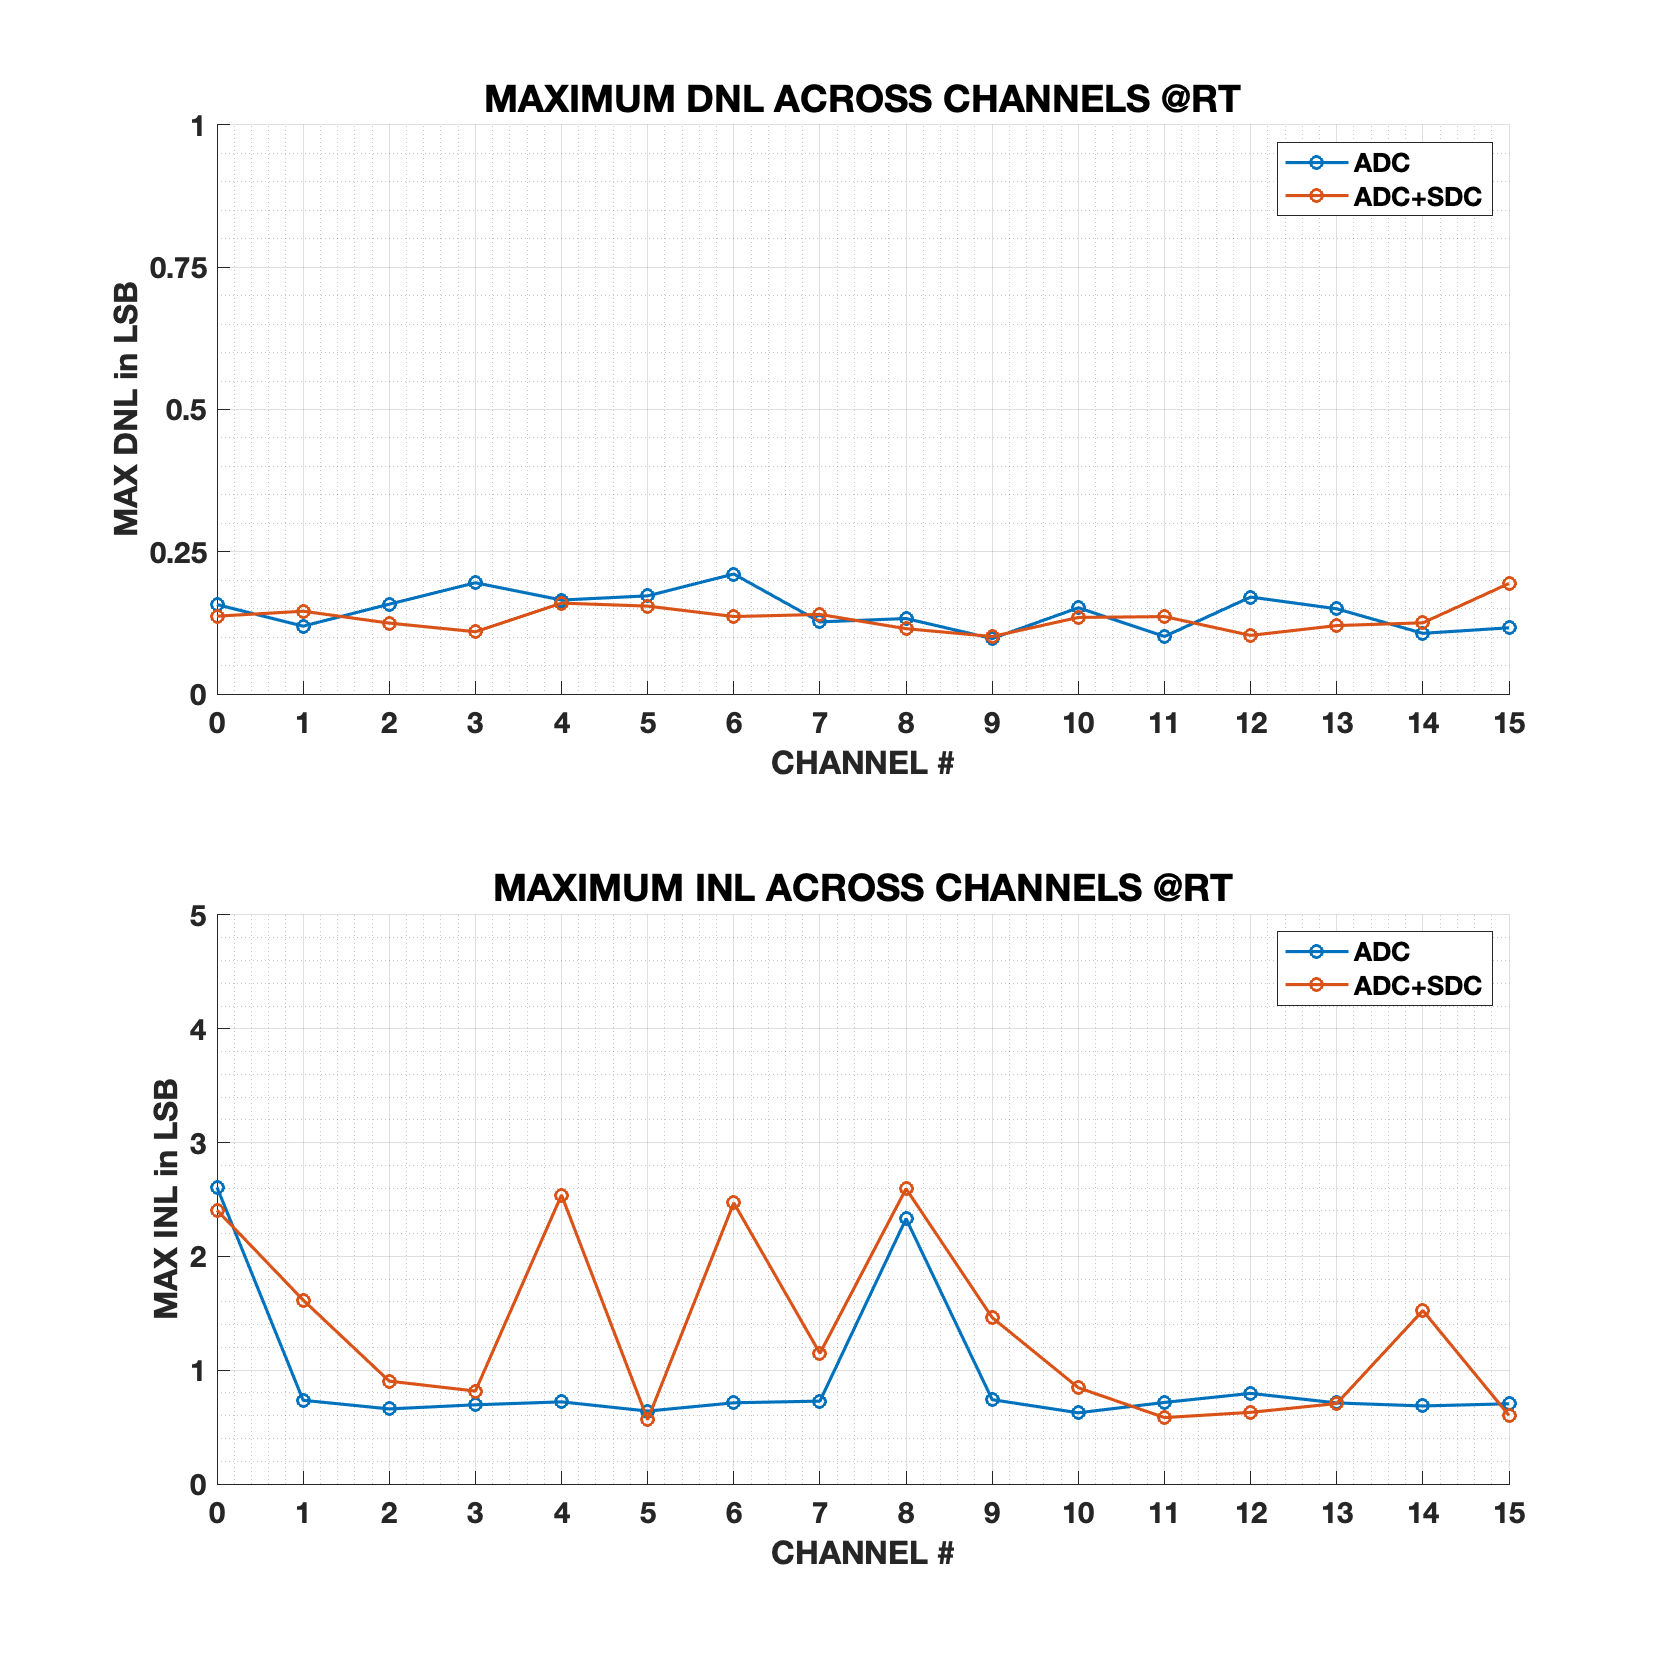
\includegraphics[width=1\linewidth]{figures/sdc_measurements/dnl_inl_ch_all_RT.png}
  \captionof{figure}{Maximum DNL and INL across ADC channels at room temperature.}
  \label{fig;sdc;inl_dnl_max_rt}
\end{minipage}
\hspace{0.2cm}
\begin{minipage}{.5\textwidth}
  \centering
  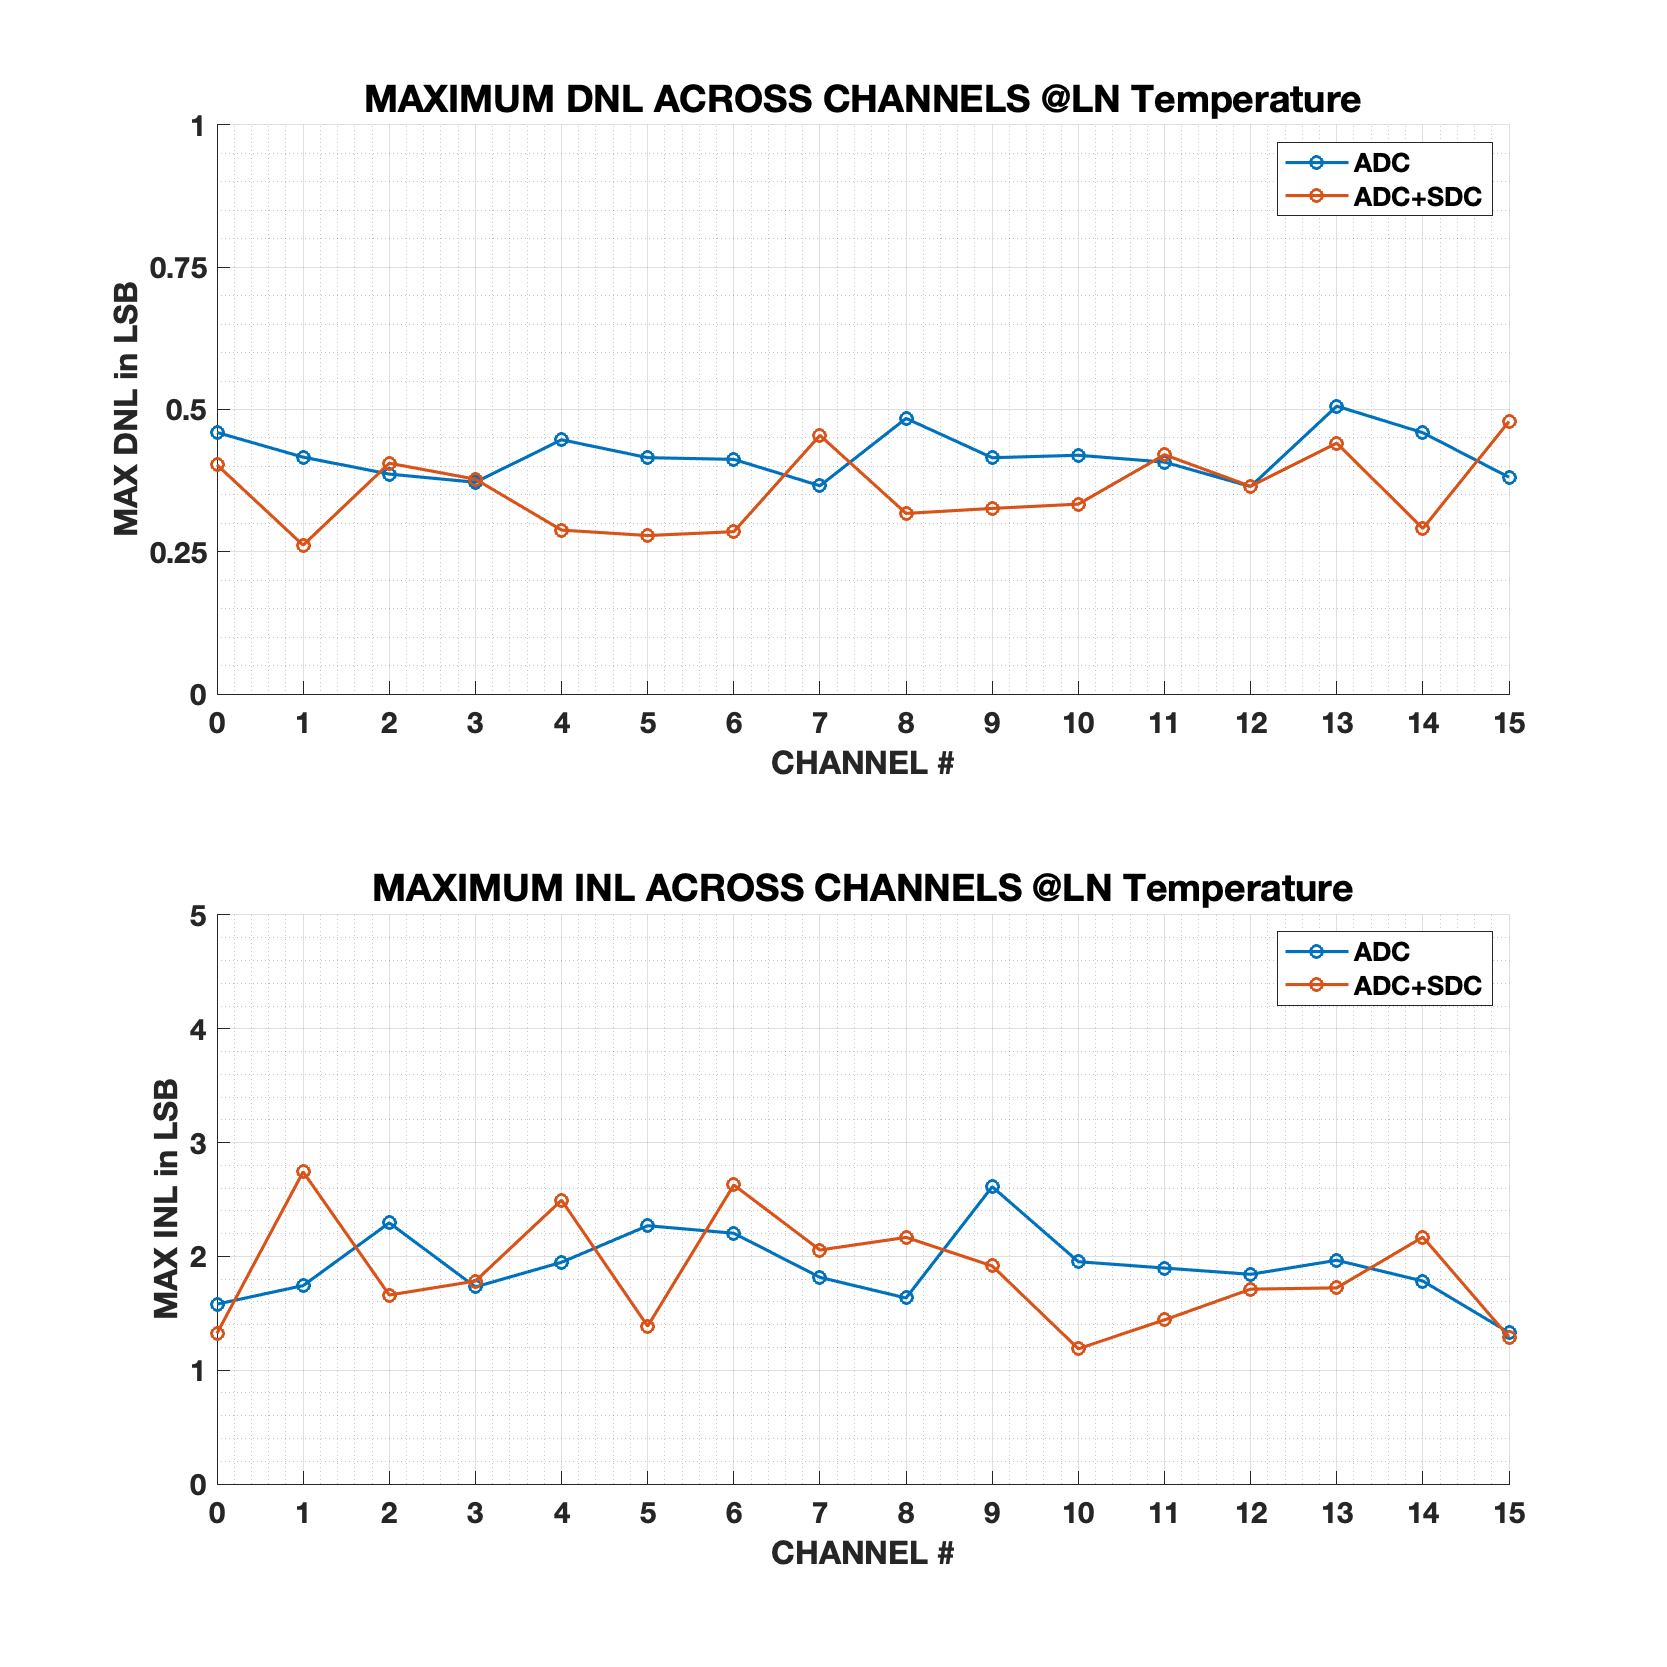
\includegraphics[width=1\linewidth]{figures/sdc_measurements/dnl_inl_ch_all_LN.png}
  \captionof{figure}{Maximum DNL and INL across ADC channels at liquid nitrogen temperature.}
  \label{fig;sdc;inl_dnl_max_ln}
\end{minipage}
\end{figure}

\begin{figure}[ht!]
  \centering
  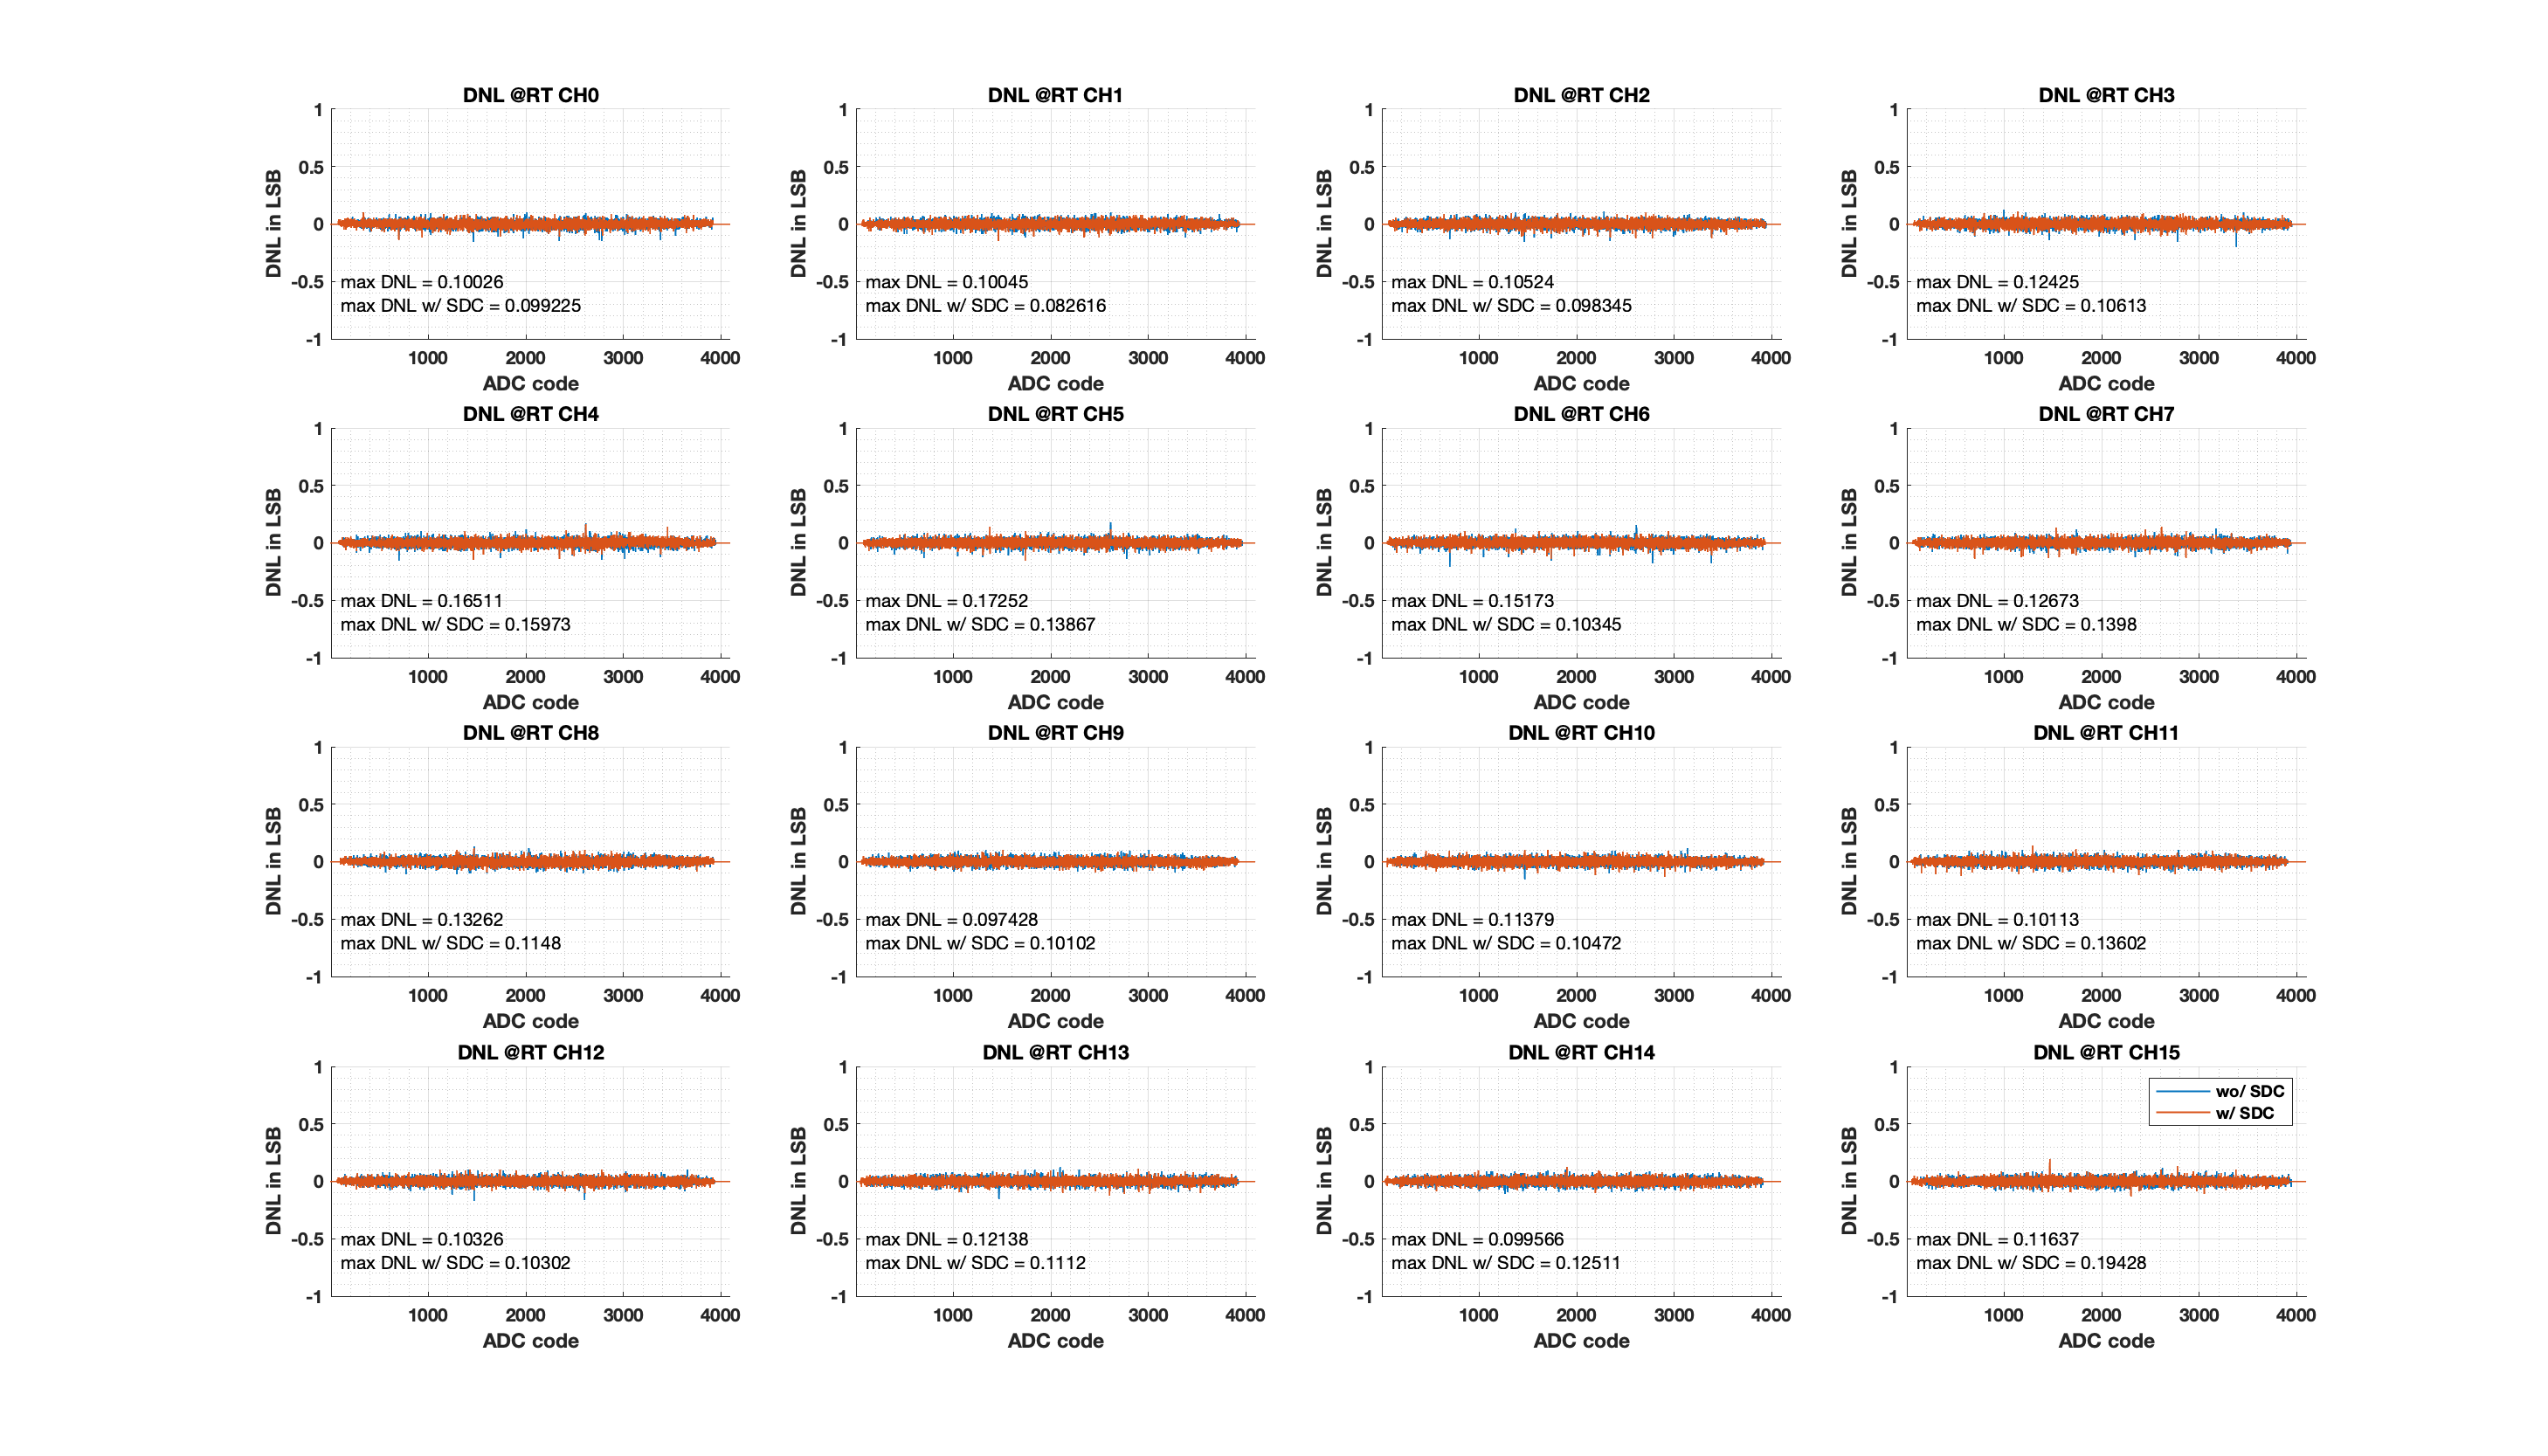
\includegraphics[width=1\linewidth]{figures/sdc_measurements/dnl_vs_dnl_sdc_all_ch_RT.png}
  \caption{Measurement of DNL across all ADC channels at room temperature. Blue - SDC off, Orange - SDC on.}
  \label{fig;sdc;dnl_all_rt}
\end{figure}

\begin{figure}[ht!]
  \centering
  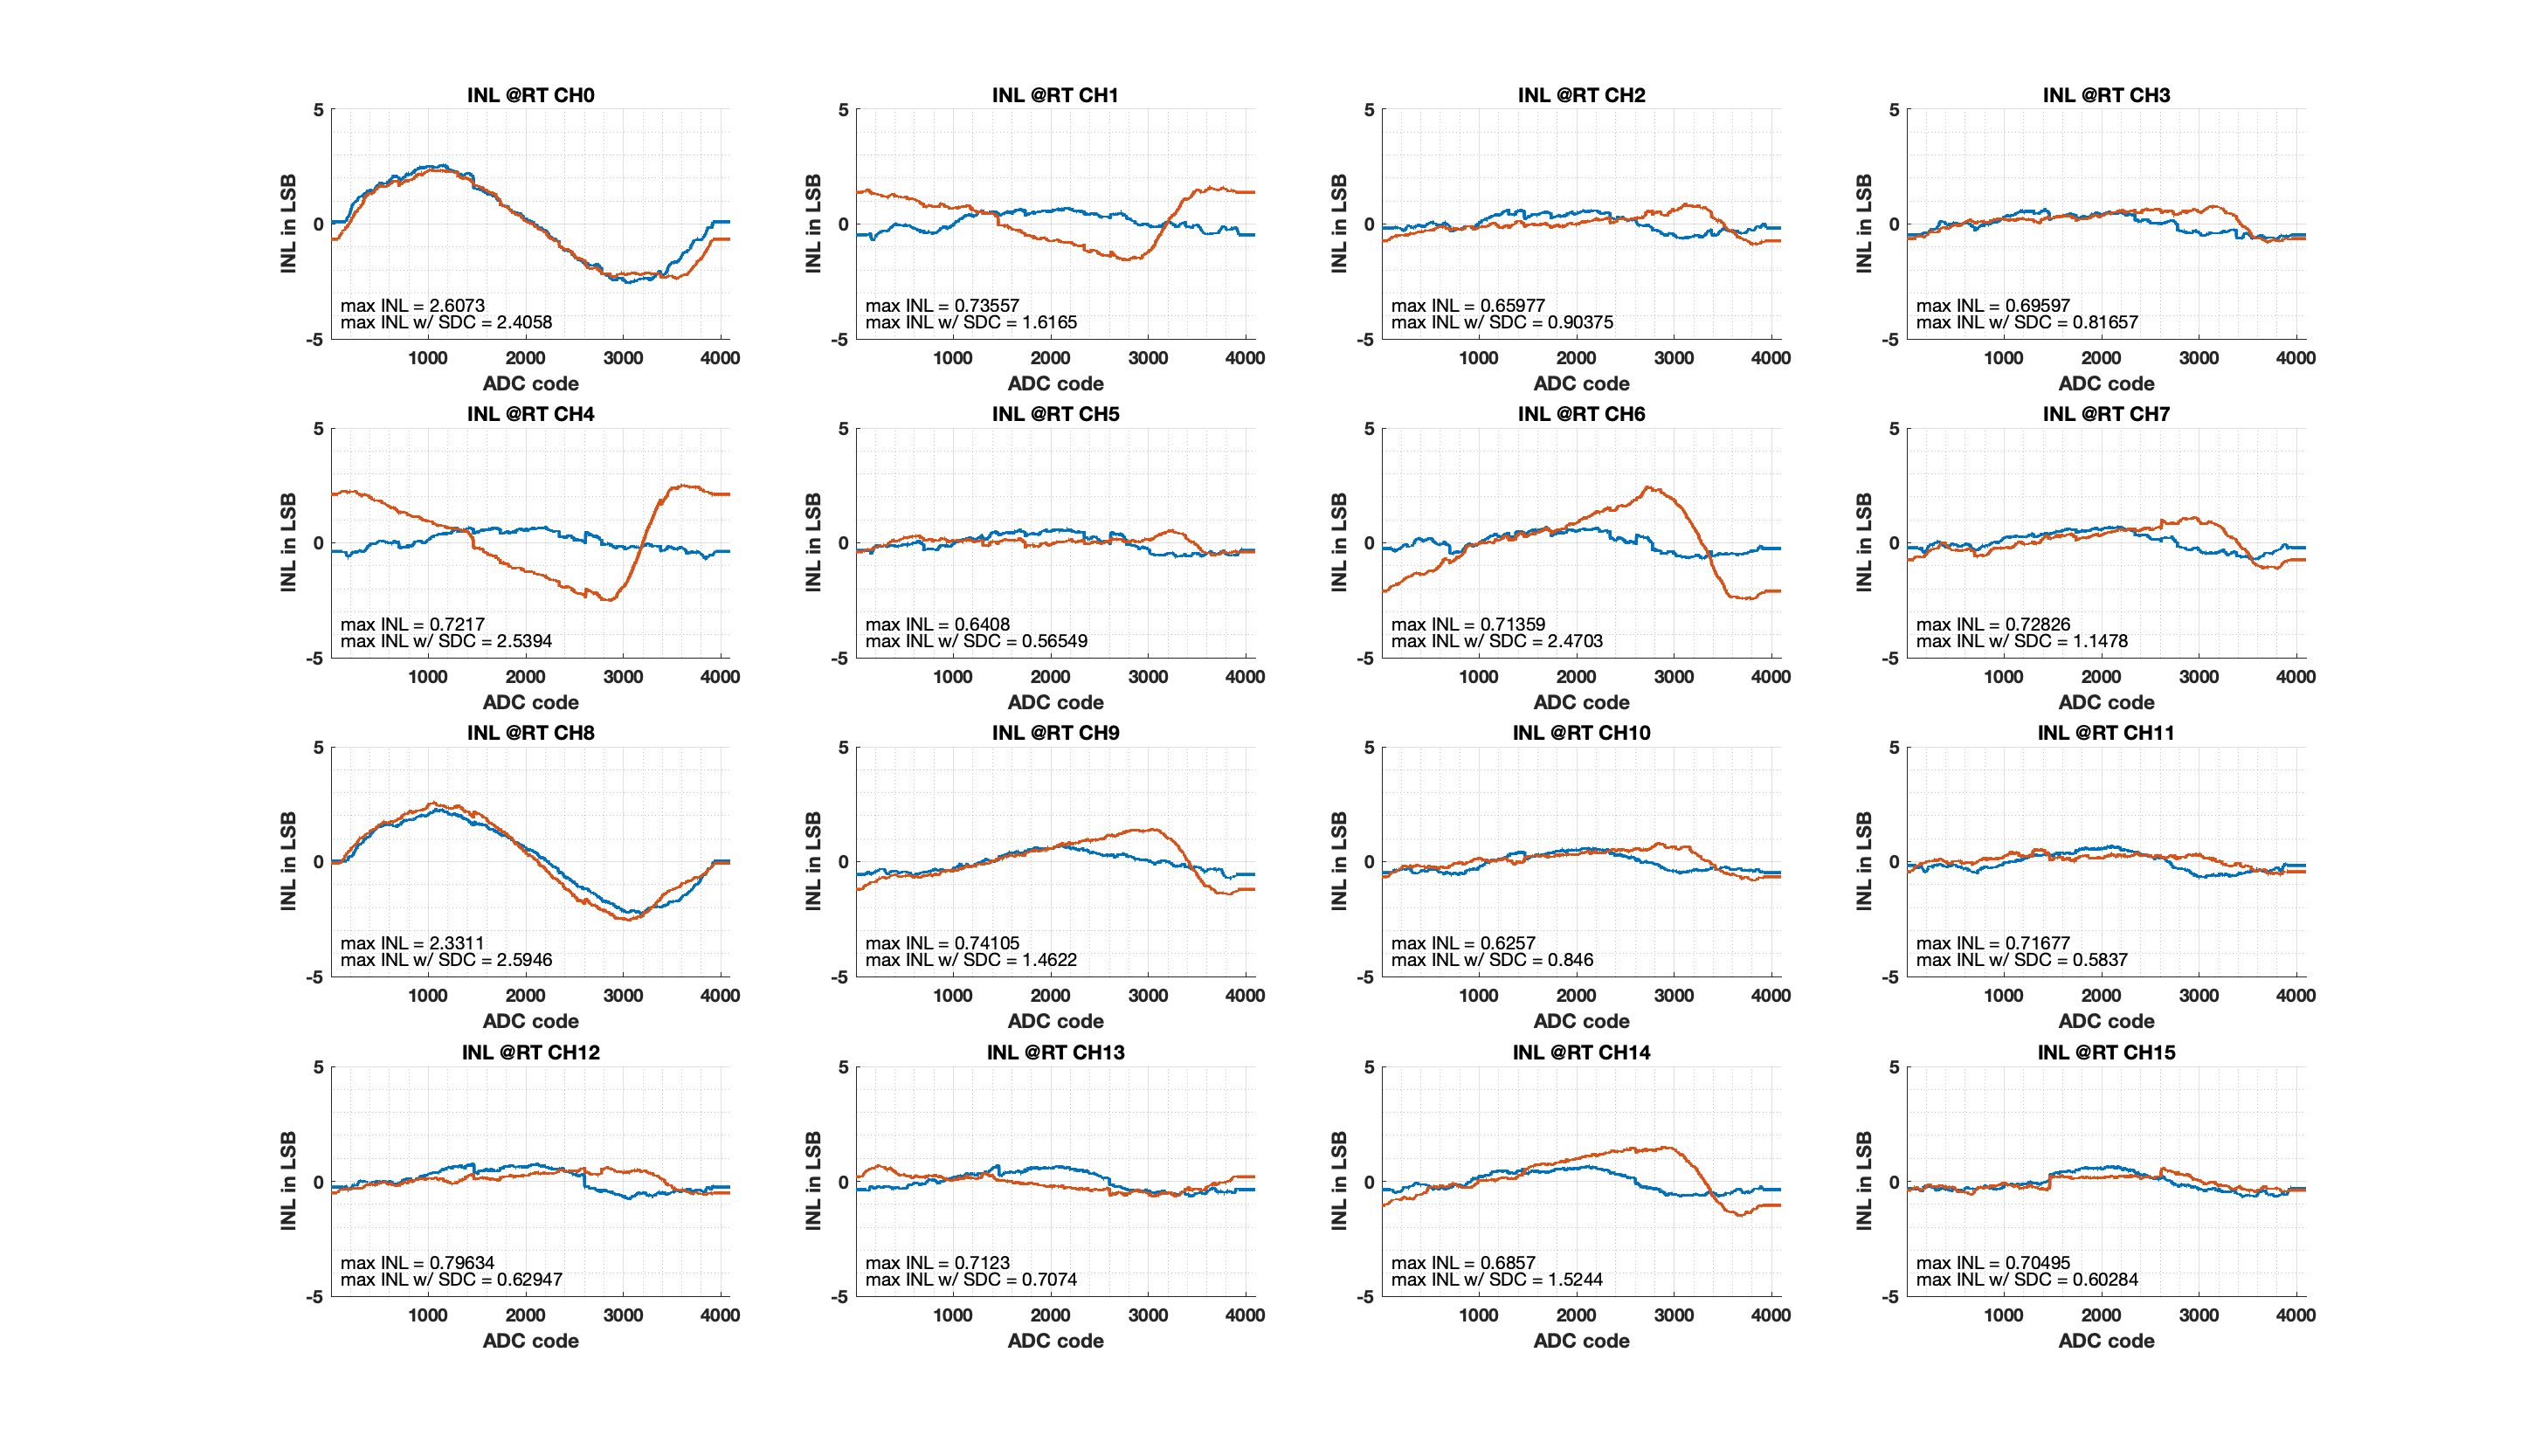
\includegraphics[width=1\linewidth]{figures/sdc_measurements/inl_vs_inl_sdc_all_ch_RT.png}
  \caption{Measurement of INL across all ADC channels at room temperature. Blue - SDC off, Orange - SDC on.}
  \label{fig;sdc;inl_all_rt}
\end{figure}

\begin{figure}[ht!]
  \centering
  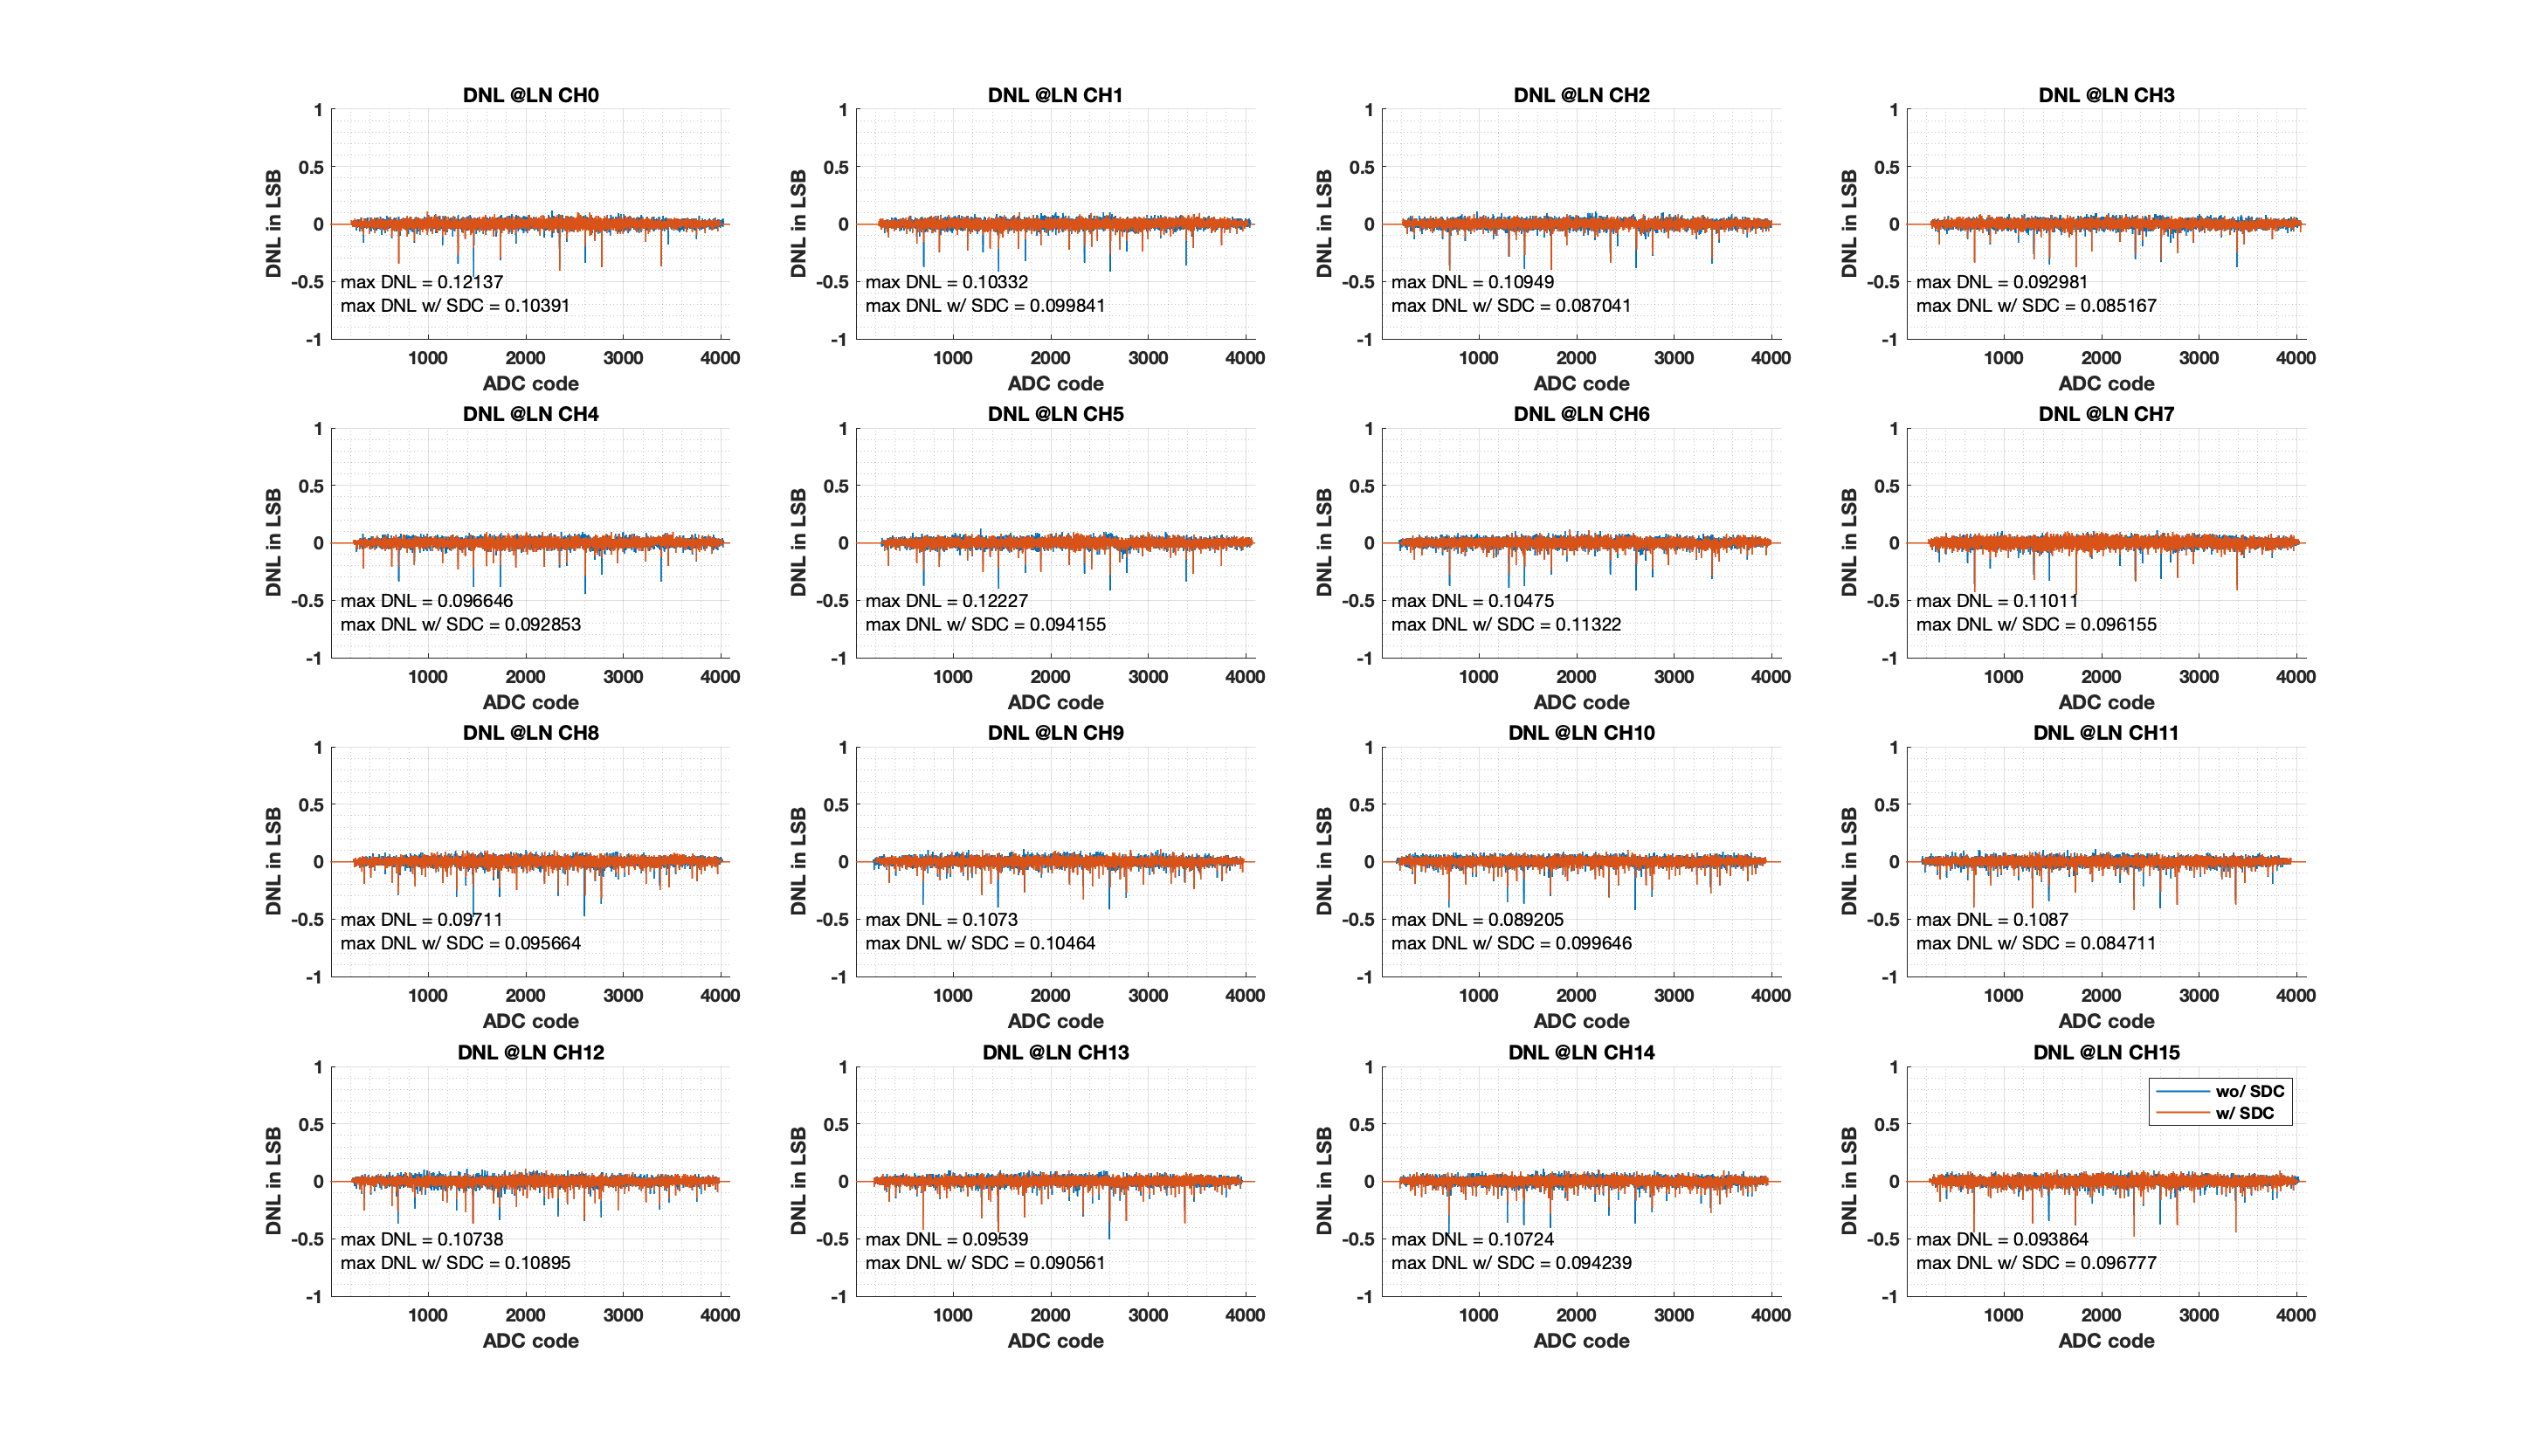
\includegraphics[width=1\linewidth]{figures/sdc_measurements/dnl_vs_dnl_sdc_all_ch_LN.png}
  \caption{Measurement of DNL across all ADC channels at liquid nitrogen temperature. Blue - SDC off, Orange - SDC on.}
  \label{fig;sdc;dnl_all_ln}
\end{figure}

\begin{figure}[ht!]
  \centering
  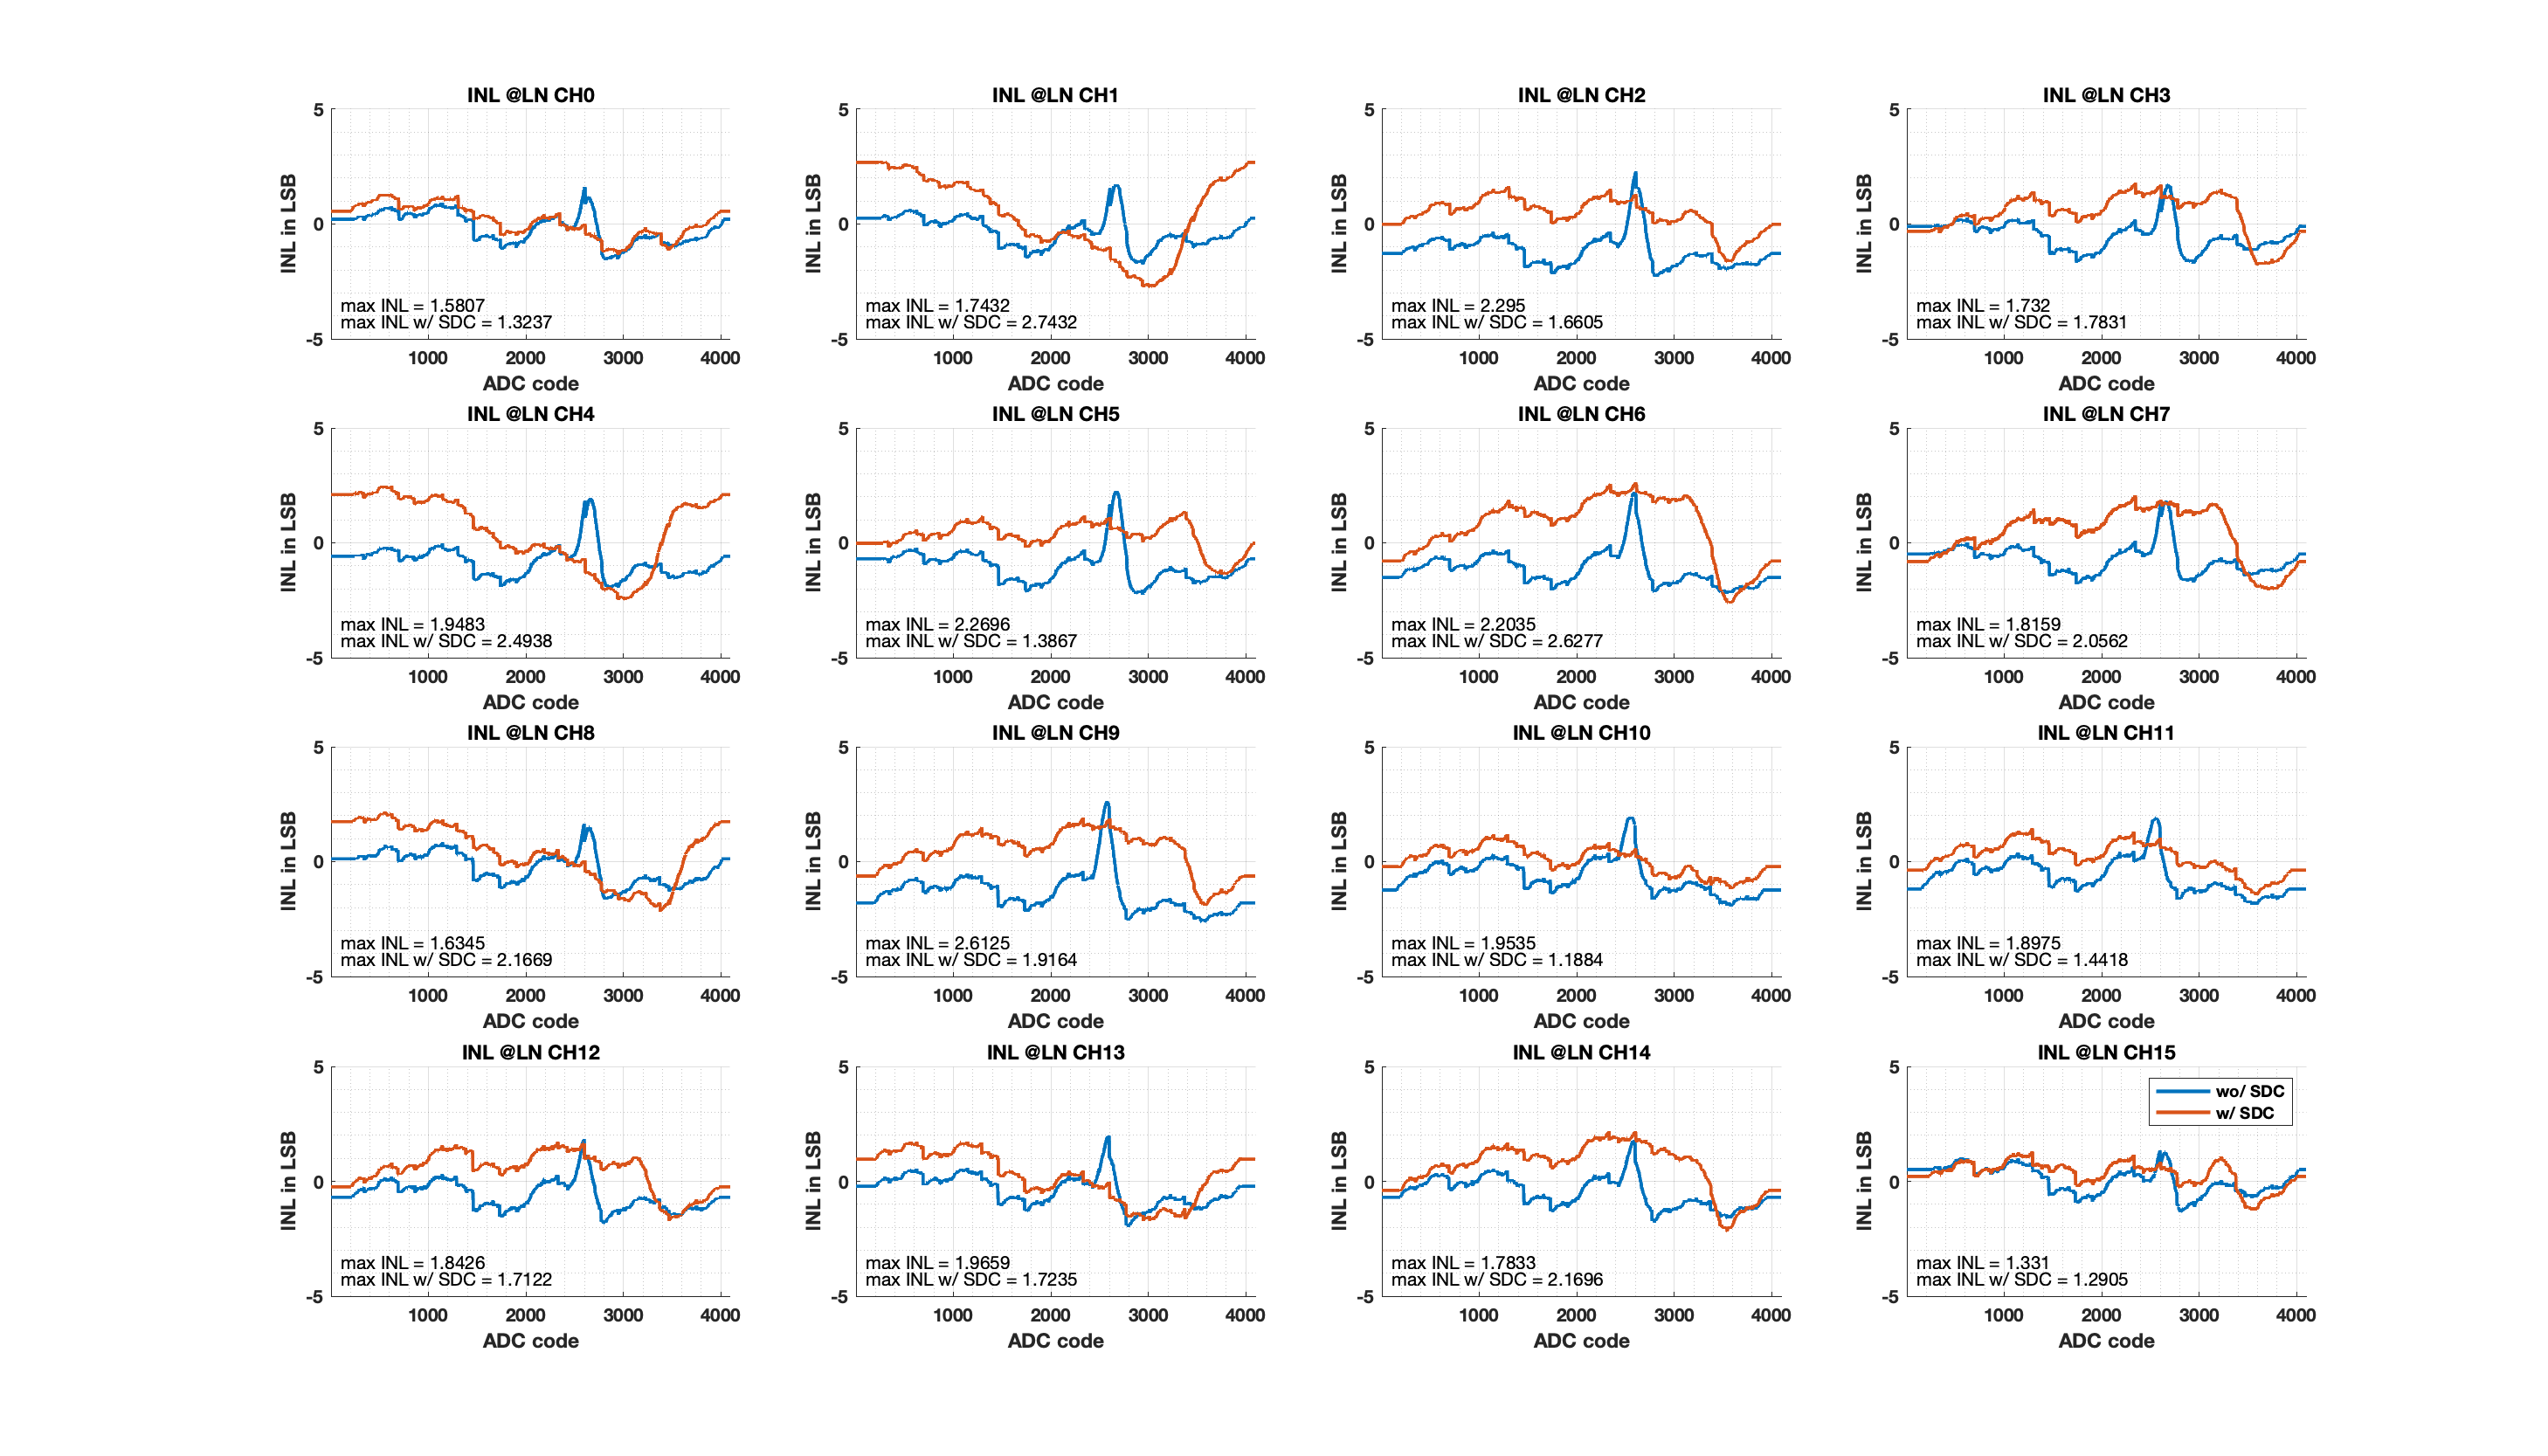
\includegraphics[width=1\linewidth]{figures/sdc_measurements/inl_vs_inl_sdc_all_ch_LN.png}
  \caption{Measurement of INL across all ADC channels at liquid nitrogen temperature. Blue - SDC off, Orange - SDC on.}
  \label{fig;sdc;inl_all_ln}
\end{figure}

\begin{figure}[ht!]
  \centering
  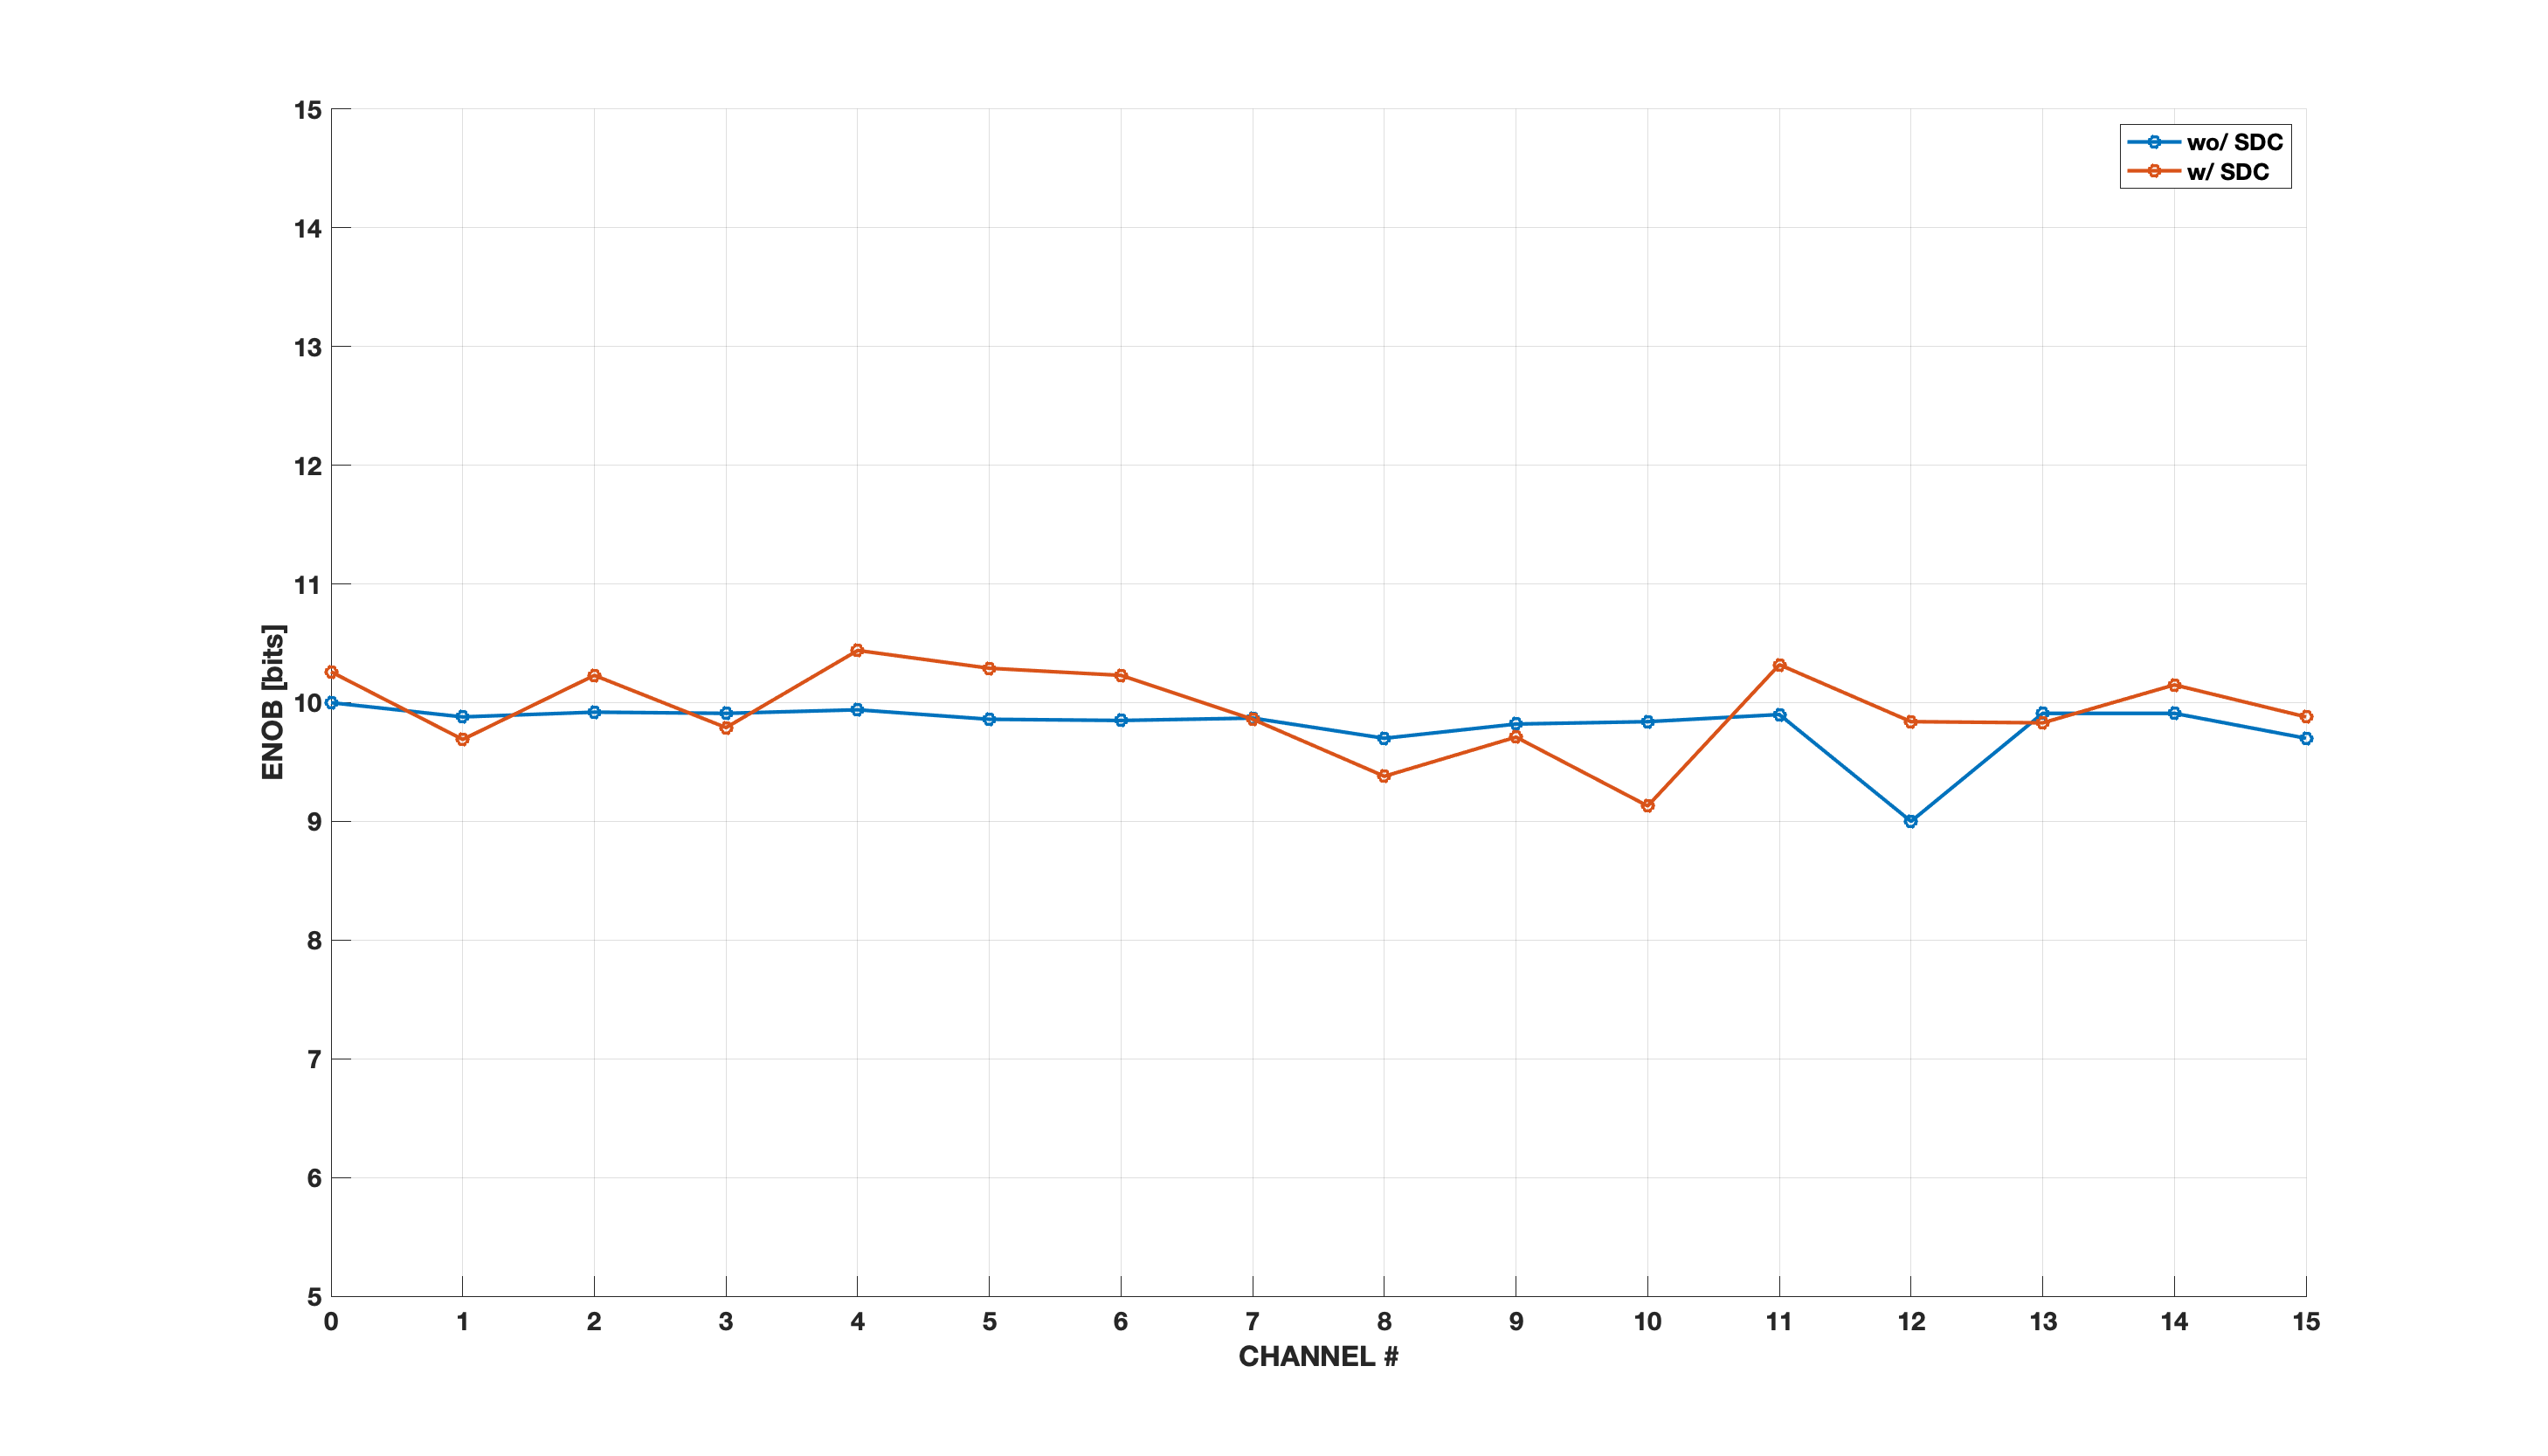
\includegraphics[width=1\linewidth]{figures/sdc_measurements/enob_rt.png}
  \caption{Measurement of ENOB across all ADC channels at room temperature.}
  \label{fig;sdc;enob_rt}
\end{figure}

\newpage
\clearpage
